% Alternative Options:
%	Paper Size: a4paper / a5paper / b5paper / letterpaper / legalpaper / executivepaper
% Duplex: oneside / twoside
% Base Font Size: 10pt / 11pt / 12pt
\documentclass[a4paper, twoside, 11pt]{report}


% This file contains all the packages used in the template
% Remove or add new packages to suit your needs




%% Language %%%%%%%%%%%%%%%%%%%%%%%%%%%%%%%%%%%%%%%%%%%%%%%%%

% Bytt til norsk for å få norsk innholdsfortegnelse
\usepackage[USenglish]{babel} % norsk, francais, polish, spanish, ...

\usepackage[utf8]{inputenc}
\usepackage[T1]{fontenc}

%% Andre pakker %%%%%%%%%%%%%%%%%%%%%%%%%%%%%%%%%%%%%%%%%%%%%%%%%
\usepackage{hyperref}
\usepackage{biblatex}
\usepackage{csquotes}
\usepackage{graphicx} %%For loading graphic files
\usepackage{amsmath}
\usepackage{amsthm}
\usepackage{amsfonts}
\usepackage{eso-pic}
\usepackage{transparent}
\usepackage{times}




%\usepackage{auto-pst-pdf} % Enables the psfrag tool
%\usepackage{psfrag}% Enables the psfrag tool
\usepackage{psfrag}
\usepackage{authblk}


%% For programming text input %%%%%%%%%%%%%%%%%%%%%%%%%%%%%%%%%%%%%%%%%%%%%%%%%

\usepackage[framed,numbered,autolinebreaks,useliterate]{mcode}
\usepackage{listingsutf8}
% Small fix for special characters
\lstset{literate=
  {á}{{\'a}}1 {é}{{\'e}}1 {í}{{\'i}}1 {ó}{{\'o}}1 {ú}{{\'u}}1
  {Á}{{\'A}}1 {É}{{\'E}}1 {Í}{{\'I}}1 {Ó}{{\'O}}1 {Ú}{{\'U}}1
  {à}{{\`a}}1 {è}{{\`e}}1 {ì}{{\`i}}1 {ò}{{\`o}}1 {ù}{{\`u}}1
  {À}{{\`A}}1 {È}{{\'E}}1 {Ì}{{\`I}}1 {Ò}{{\`O}}1 {Ù}{{\`U}}1
  {ä}{{\"a}}1 {ë}{{\"e}}1 {ï}{{\"i}}1 {ö}{{\"o}}1 {ü}{{\"u}}1
  {Ä}{{\"A}}1 {Ë}{{\"E}}1 {Ï}{{\"I}}1 {Ö}{{\"O}}1 {Ü}{{\"U}}1
  {â}{{\^a}}1 {ê}{{\^e}}1 {î}{{\^i}}1 {ô}{{\^o}}1 {û}{{\^u}}1
  {Â}{{\^A}}1 {Ê}{{\^E}}1 {Î}{{\^I}}1 {Ô}{{\^O}}1 {Û}{{\^U}}1
  {Ã}{{\~A}}1 {ã}{{\~a}}1 {Õ}{{\~O}}1 {õ}{{\~o}}1
  {œ}{{\oe}}1 {Œ}{{\OE}}1 {æ}{{\ae}}1 {Æ}{{\AE}}1 {ß}{{\ss}}1
  {ű}{{\H{u}}}1 {Ű}{{\H{U}}}1 {ő}{{\H{o}}}1 {Ő}{{\H{O}}}1
  {ç}{{\c c}}1 {Ç}{{\c C}}1 {ø}{{\o}}1 {å}{{\r a}}1 {Å}{{\r A}}1
  {€}{{\euro}}1 {£}{{\pounds}}1 {«}{{\guillemotleft}}1
  {»}{{\guillemotright}}1 {ñ}{{\~n}}1 {Ñ}{{\~N}}1 {¿}{{?`}}1
}


%% Line Spacing %%%%%%%%%%%%%%%%%%%%%%%%%%%%%%%%%%%%%%%%%%%%%
%\usepackage{setspace}
%\singlespacing        %% 1-spacing (default)
%\onehalfspacing       %% 1,5-spacing
%\doublespacing        %% 2-spacing


%% Other Packages %%%%%%%%%%%%%%%%%%%%%%%%%%%%%%%%%%%%%%%%%%%
%\usepackage{a4wide} %%Smaller margins = more text per page.
\usepackage{fancyhdr} %%Fancy headings
%\usepackage{longtable} %%For tables, that exceed one page

\usepackage{color}
\definecolor{darkgreen}{rgb}{0.3,0.6,0.3}

\parindent 0mm
\setlength{\oddsidemargin}{0mm}
\setlength{\evensidemargin}{0mm}
\setlength{\topmargin}{-20mm}
\setlength{\textwidth}{165mm}
\setlength{\textheight}{260mm}

\hypersetup{
   pdfauthor={UiA Mechatronics Student},
   pdftitle={Technical Report},
   pdfkeywords={report, mechatronics, University of Agder},
   pdfsubject={Project Report},
   colorlinks=true,
   citecolor=darkgreen,
   urlcolor=darkgreen,
   linkcolor=black,
   pdfstartview=Fit,
   pdfpagelayout=SinglePage,
   pdfcreator=pdflatex,
   pdfproducer=pdflatex
}


\addbibresource{bibliography.bib}

\begin{document}
%\rmfamily




\pagestyle{empty} %No headings for the first pages.


\begin{titlepage}
    \vbox{ }

    \vbox{ }

    \begin{center}
        % Øverste del av siden
        
\includegraphics[width=0.6\textwidth]{Figures/Frontpage/tekreal}\\[4cm]
        \textsc{\Large IKT115 - Introduksjon til kunstig intelligens-teknologi}\\[0.7cm]

        % \vbox{ }
        % Tittel
        \noindent\makebox[\linewidth]{\rule{.7\paperwidth}{.6pt}}\\[0.7cm]
        { \huge \bfseries Fordypningsoppgave}\\[0.25cm]
        \noindent\makebox[\linewidth]{\rule{.7\paperwidth}{.6pt}}\\[0.7cm]
        \large{Spring 2024}\\[1.2cm]
        \vfill
        % Forfatter
        \large
        % \emph{Skrevet av:}\\[1mm]
        Gormery K. Wanjiru

        % Nederste del av siden
        {\large \today}
    \end{center}
\end{titlepage}
  
\clearpage

\pagenumbering{gobble}
\pagenumbering{roman}


\newpage



\large{\bf{Obligatorisk gruppeerklæring}} \\

{\small \hbadness=10000
Den enkelte student er selv ansvarlig for å sette seg inn i hva som er lovlige hjelpemidler, retningslinjer for bruk av disse og regler om kildebruk. Erklæringen skal bevisstgjøre studentene på deres ansvar og hvilke konsekvenser fusk kan medføre. Manglende erklæring fritar ikke studentene fra sitt ansvar.\\

\begin{center}
\begin{tabular}{ |p{1cm}|p{11.5cm}|p{1cm}|}
 \hline  
 
 1. & Vi erklærer herved at vår besvarelse er vårt eget arbeid, og at vi ikke har brukt andre kilder eller har mottatt annen hjelp enn det som er nevnt i besvarelsen. & Ja \\
 \hline
 2. & \textbf{Vi erklærer videre at denne besvarelsen:}
 \begin{itemize}
    \item Ikke har vært brukt til annen eksamen ved annen avdeling/universitet/høgskole innenlands eller utenlands.
    \item Ikke refererer til andres arbeid uten at det er oppgitt.
    \item Ikke refererer til eget tidligere arbeid uten at det er oppgitt.
    \item Har alle referansene oppgitt i litteraturlisten.
    \item Ikke er en kopi, duplikat eller avskrift av andres arbeid eller besvarelse.
 \end{itemize}& Ja \\
 \hline
 3. & Vi er kjent med at brudd på ovennevnte er å betrakte som fusk og kan medføre annullering av eksamen og utestengelse fra universiteter og høgskoler i Norge, jf. Universitets- og høgskoleloven §§4-7 og 4-8 og Forskrift om eksamen §§ 31.
 & Ja \\
 \hline
 4. & Vi er kjent med at alle innleverte oppgaver kan bli plagiatkontrollert.
 & Ja \\
 \hline
 5. & Vi er kjent med at Universitetet i Agder vil behandle alle saker hvor det forligger mistanke om fusk etter høgskolens retningslinjer for behandling av saker om fusk.
 & Ja \\
 \hline
 6. & Vi har satt oss inn i regler og retningslinjer i bruk av kilder og referanser på biblioteket sine nettsider.
 & Ja \\
 \hline
 7. & Vi har i flertall blitt enige om at innsatsen innad i gruppen er merkbart forskjellig og ønsker dermed å vurderes individuelt.
Ordinært vurderes alle deltakere i prosjektet samlet.
 & Ja \\
 \hline
\end{tabular}
\end{center}}

\bigskip

\large{\bf{Publiseringsavtale}} \\

{\small \hbadness=10000 Fullmakt til elektronisk publisering av oppgaven
Forfatter(ne) har opphavsrett til oppgaven. Det betyr blant annet enerett til å gjøre verket tilgjengelig for allmennheten (Åndsverkloven. §2).
\\
Oppgaver som er unntatt offentlighet eller taushetsbelagt/konfidensiell vil ikke bli publisert.\\

\begin{center}
\begin{tabular}{ |p{13cm}|p{1cm}|}
\hline
Vi gir herved Universitetet i Agder en vederlagsfri rett til å gjøre oppgaven tilgjengelig for elektronisk publisering: & Ja \\
\hline
Er oppgaven båndlagt (konfidensiell)? & Nei \\
\hline
Er oppgaven unntatt offentlighet? & 
Nei \\
\hline
\end{tabular}
\end{center}
}


\chapter*{Acknowledgements}
This template is meant as an example of how a technical report can be structured. Discuss
the table of content and the names of the chapters with the group members and supervisor
to suit your specific report.


\addcontentsline{toc}{chapter}{Acknowledgements}

\clearpage
\chapter*{Abstract}
My field of study is Artificial Intelligence, 5-year master programme. I've always been interested in AI and that is why i study it. Most of the thing in this report are my own meaning that i've honed over the years. This also means that it may be inspired by articles, videos, and people through out my life(since i was 13). Some so long ago i can't possibly remember where i heard it from to reference it.
\addcontentsline{toc}{chapter}{Abstract}

\clearpage

\tableofcontents
\cleardoublepage %The first chapter should start on an odd page.
\pagestyle{plain} %Now display headings: headings / fancy / ...

%List of Figures
\listoffigures
\addcontentsline{toc}{chapter}{List of Figures}
\clearpage
\textcolor{white}{.}
\thispagestyle{empty}
\newpage

%List of Tables
\listoftables
\addcontentsline{toc}{chapter}{List of Tables}
\clearpage

\textcolor{white}{.}
\thispagestyle{empty}
\newpage

\clearpage
\pagenumbering{arabic}





\chapter{Introduction}
Image recognition is big field within ai that has perhaps the most noticable results. While today LLM are what are most famous today, you could say right before openai released gpt3 and further back, image recognition was what carried the ai interest baggage. Most people before then, including myself probably got intreseted and decided to study AI because of image recognistion. perhaps they saw something done and fell i love or thay needed a physical world task done etc.




\chapter{Theory and Goals}
The image recognition im going to make is animal recognition. It is a simple project but can truly showcase the abilities of model, the affects of the training and how good the results are.

This is because Animals are diverse. They come in all different  shapes and sized and also similar shapes and sizes. The model would be good if it can differentiate different shape and size animals but even better is it can differentiate similar ones. That is the goal.

Some categories its going to me trained on are varied from pets, to safari animals, asian animals ets. 

The model we used is called animal-data\cite{animal-data} and it came from kaggle.

The datasets contains realatively good quality images and for each image it has different oriantations, brightness and reflections of it. this makes made the data set even more valuable as ut could gave four different pictures from the same picture.
here are some example images in the mode:

\begin{figure}[h]
    \centering
    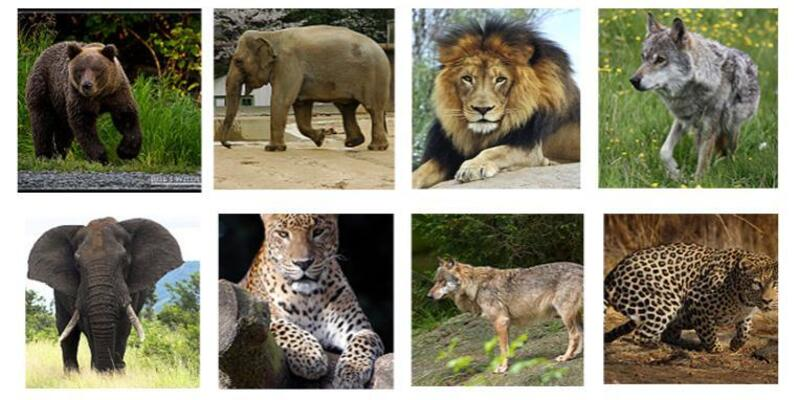
\includegraphics[width = 0.7\textwidth]{Figures/img/dataset-cover.png}
    \caption{Cover image of the animal-data\cite{animal-data} dataset on kaggle}
    \label{fig:label1}
\end{figure}
\chapter{Methods in ...}
\chapter{Results}
\subsection{Results and Discussion}
So, I sent in at it at least 12 images for each category, just to see the basic stats like accuracy, and confidence. What do you know? It nailed the accuracy on the training set images—like a perfect 100\%. It's good at what it learned, which was to be expected. But then, it was time to make this more interesting, let’s make this a bit more interesting. 

I tested it with some tricky images from Google, trying to trip it up a bit, and true? It stumbled sometimes. I used images of asses mostly but placed them in different settings to really push the limits. When the background was grassy or dry, the model thought the donkey was a kangaroo. When there was a noticeable hanging stomach, it guessed cow, and with mountainous or forest backgrounds, it went with deer. Interestingly, it never guessed horse, which would be the closest. So i investigated the training data for horses a bit. Turns out, in the training set, the horses were mostly either vibrant brown or white - and other vibrant colors, never the grey shades like those of a donkey. This little experiment showed the model does what it’s supposed to—extract features and recognize them, but only within the context it was trained on.

When it comes tweaking things. I played around with different settings in the "Advanced" options—things like tweaking the number of training epochs. Increasing the epochs did bump up the accuracy initially, but then it plateaued, and going too long actually started to hurt the performance. This is the same with what I've learned about potential overfitting—too much learning isn't always a good thing.

\subsubsection{What Worked and What Didn't}
I have a few examples to show this off:
\begin{itemize}
    \item \textbf{correct clasification:} There were cases where the model was spot on. I’ll put those images right here in the report, and you can see how it got them right. it was the very different animals like birds, elephant etc.
    \item \textbf{Misclassifications:} Then there were the misfires. Like the donkey-dressed-as-a-deer kind of mistakes. I’ll show these too, along with a discussion on why it probably messed up. the similar animals like deer, horse and shockingly kangaroo
    \item \textbf{Weird Stuff:} And for fun, I threw in some totally unrelated images just to see what it would do. The results were as mentioned before
\end{itemize}

\subsubsection{Ethical and Practical Challenges}
Discussing ethics,
Here are three ethical challenges with this model:
\begin{enumerate}
    \item \textbf{Bias in Training Data:}
    \item \textbf{Misuse of Technology:}
    \item \textbf{Data Privacy:} Where and how we source our images could should be thought about extensively.
\end{enumerate}

this model has big potentions here are some just to mention afew:
\begin{enumerate}
    \item More diverse data, especially with color variations.
    \item Maybe tweaking the neural network architecture itself, adding some layers or playing around with the dropout rate.
    \item also better curating of data. like in the case of hose i dint notice until the model was trained because the issue with the data what unnoticable normally
\end{enumerate}

our model is decent at recognizing stuff, as long as it's stuff it has seen in somewhat similar contexts before. But throw something different, and it’s a bit of a coin toss.

\chapter{Discussions}
\chapter{Conclusions}
when I added more images to the training dataset, the model's performance improved. More data, better learning, who would've thought, right?

generally a good learning experience


\appendix

\chapter{Use of AI:}

Locations:  https://chat.openai.com\\
Model: GPT4
\\

it was only used as shown in the text section 2.2.1 and no edits were used to the response except space indentation in latex.
The incorrect vocabulary it there by design to show case that ai understands even if the input is incorrect. Also to simulate vocal commands


\printbibliography[
heading=bibintoc,
title={Bibliography}
]

\end{document}

